\documentclass{article}
\usepackage{paquetes/caratula}
\usepackage[a4paper, left=2.5cm, right=2.5cm, bottom=2.5cm, top=3.0cm]{geometry}
\usepackage{indentfirst}
\usepackage{graphicx}
\usepackage{subcaption}
\usepackage{amsmath}
\usepackage{amssymb}
\usepackage{xcolor}
\usepackage{float}
\usepackage{graphicx}


\makeindex


\begin{document}

\titulo{Trabajo Práctico 1}
\subtitulo{Programación Lineal}
\fecha{1$^{\text{er}}$ cuatrimestre 2025}
\materia{Investigación Operativa}

\integrante{Guibaudo, Camila}{682/17}{camiguiba@gmail.com}
\integrante{Azar, Agustin}{693/21}{Agustin.azar101@gmail.com}
\integrante{Pages, Julieta}{1691/21}{julib.pages@gmail.com}

\maketitle

\newpage

%%%%%%%%%%%%%%%%%%%%%%%%%%%%%%%%%%%%%%%%%%%%%%%%%%%%%%%%%%%%%%%%%%%%%%%%%%%%%%%%%%%%%%%%%%%%
%%%%%%%%%%%%%%%%%%%%%%%%%%%%%%         Modelos de PE      %%%%%%%%%%%%%%%%%%%%%%%%%%%%%%%%%%
%%%%%%%%%%%%%%%%%%%%%%%%%%%%%%%%%%%%%%%%%%%%%%%%%%%%%%%%%%%%%%%%%%%%%%%%%%%%%%%%%%%%%%%%%%%%
\section{Modelos}
Se nos presentó un problema donde una empresa debe distribuir productos a varios clientes, y quiere incorporar una nueva metodología para hacerlo. Entonces, para ver si podría ser conveniente, se desarrollaron tres modelos. El primero para representar el modelo actual de distribución, que coincide con el modelo del \textit{The Traveling Salesman Problem}, así podemos ver el costo óptimo actual. Luego se realizó un modelo que pasa a incluir la opción de realizar ciertas entregas en bici desde un punto por el que pasara el camión, sujeto a ciertas restricciones. Y por último, vamos a tener un tercer modelo que consiste en agregar al modelo anterior un par de restricciones que serían deseables, y nos interesa ver cuánto se perdería en caso de tenerlas en cuenta. 

%%%%%%%%%%%%%%%%%%%%%%%%%%%%%%         TSP      %%%%%%%%%%%%%%%%%%%%%%%%%%%%%%%%%%
\subsection{Modelo de la metodología actual (TSP):} \label{modelo_actual}
\subsection*{Variables}
\begin{align*}
    x_{i\_j} &\in \{0,1\} && \text{1 si se viaja del nodo } i \text{ al nodo } j \\
    u_i &\in \mathbb{R} && \text{Variable auxiliar para eliminación de subciclos (MTZ)}
\end{align*}

\subsection*{Restricciones}

\paragraph{1. Visitar una única vez cada cliente}
\[
\sum_{j=1}^{n} x_{ij} = 1 \quad \forall i \in \{1, \dots, n\}
\]

\paragraph{2. Conservación de flujo}
\[
\sum_{\substack{j=1 \\ j \ne i}}^{n} x_{ij} - \sum_{\substack{j=1 \\ j \ne i}}^{n} x_{ji} = 0 \quad \forall i \in \{1, \dots, n\}
\]

\paragraph{3. Eliminación de subciclos / detour (MTZ)}
\[
u_i - u_j + (n - 1)x_{ij} \leq n - 2 \quad \forall i, j \in \{2, \dots, n\},\ i \ne j
\]

\[
u_1 = 0
\]

\[
1 \leq u_i \leq n - 1 \quad \forall i \in \{2, \dots, n\}
\]

%%%%%%%%%%%%%%%%%%%%%%%%%%%%%%         Nuevo Modelo      %%%%%%%%%%%%%%%%%%%%%%%%%%%%%%%%%%
\subsection{Modelo de la nueva metodología (agregar repartidores):} \label{model_repartidores}
\subsection*{Variables}
\begin{align*}
    x_{i\_j} &\in \{0,1\} && \text{1 si se va del nodo } i \text{ al nodo } j \text{ en camión }\\
    u_i &\in \mathbb{R} && \text{Variable auxiliar para eliminación de subciclos (MTZ)} \\
    r_{ij} &\in \{0,1\} && \text{1 si se va del nodo } i \text{ al nodo } j \text{ con repartidor (bici) } \\
    d_{i} &\in \{0,1\} && \text{1 si el nodo $i$ es depósito } 
\end{align*}

\subsection*{Parámetros}
\begin{itemize}
    \item \( n \): Número total de nodos (clientes + depósito)
    \item \( i, j \in \{1, \dots, n\} \)
    \item El nodo \(1\) representa el depósito
\end{itemize}

\subsection*{Restricciones}

\paragraph{1. Solo un depósito activo}
\[
\sum_{i=1}^{n} d_i = 1
\]

\paragraph{2. El camión pasa máximo una vez por cliente}
\[
\sum_{i=1}^{n} x_{ij} \leq 1 \quad \forall j \in \{1, \dots, n\}
\]

\paragraph{3. Conservación de flujo (camión)}
\[
\sum_{\substack{j=1 \\ j \ne i}}^{n} x_{ij} - \sum_{\substack{j=1 \\ j \ne i}}^{n} x_{ji} = 0 \quad \forall i \in \{1, \dots, n\}
\]

\paragraph{4. El repartidor solo sale de nodos por los que pasó el camión}
\[
\sum_{k=1}^{n} x_{ki} + d_i - r_{ij} \geq 0 \quad \forall i,j \in \{1, \dots, n\}
\]

\paragraph{5. Cumplir la distancia máxima para el repartidor}
\[
r_{ij} \cdot \text{dist}_{ij} \leq d_{\text{max}} \quad \forall i,j \in \{1, \dots, n\}
\]

\paragraph{6. Eliminación de subciclos / detour (MTZ)} 
\[
u_i - u_j + (n - 1) x_{ij} - n d_i - n d_j \leq n - 2 \quad \forall i \ne j,\ i,j \in \{1, \dots, n\}
\]
\begin{align*}
u_i + d_i &\geq 1 \quad \forall i \in \{1, \dots, n\} \\
u_i + n \cdot d_i &\leq n \quad \forall i \in \{1, \dots, n\}
\end{align*}
(si $i$ es el depósito ($d_i=1$) entonces no le pedimos nada)

\paragraph{7. Asegurar la visita a cada cliente}
\[
\sum_{k=1}^{n} (x_{kj} + r_{kj}) + d_j \geq 1 \quad \forall j \in \{1, \dots, n\}
\]
O llego con camión, o llego con repartidor, o soy el depósito.

\paragraph{8. Máximo una entrega refrigerada por nodo}
\[
\sum_{j \in R} r_{ij} \leq 1 \quad \forall i \in \{1, \dots, n\}
\]
donde \( R \subseteq \{1, \dots, n\} \) es el conjunto de clientes con productos refrigerados.




\subsection{Modelo de la metodología adicional (agregar 2 restricciones):} \label{modelo1}

Este modelo es una extensión del modelo anterior donde se incorporan dos restricciones extra deseables por la empresa: 
\begin{itemize}
    \item Cada repartidor contratado realiza al menos 4 entregas.
    \item Hay determinados clientes que deben ser atendidos exclusivamente por el camión.
\end{itemize}
La función objetivo, las variables y las restricciones son iguales a las del modelo anterior. Solo se agregan las siguientes variables y restricciones adicionales:

\subsection*{Variables adicionales}

\begin{align*}
    r_{i} &\in \{0,1\} && \text{1 si al menos un repartidor parte del nodo } i 
\end{align*}

\subsection*{Restricciones adicionales}

\paragraph{1. Si un repartidor parte del nodo $i$, entonces debe realizar al menos cuatro entregas}
\[
\sum_{j=1}^{n} r_{ij} - 4 \cdot r_{i} \geq 0 \quad \forall i \in \{1, \dots, n\}
\]

\paragraph{2. Si un repartidor parte del nodo $i$, entonces $r_i = 1$}
\[
\sum_{j=1}^{n} r_{ij} - n \cdot r_{i} \leq 0 \quad \forall i \in \{1, \dots, n\}
\]

\paragraph{3. Si un nodo $i$ es un cliente exclusivo, entonces un camión debe pasar por él}
\[
\sum_{j=1}^{n} x_{ij} + d_{i} \geq 1 \quad \forall i \in E
\]
donde $E$ es el conjunto de clientes exclusivos.


%%%%%%%%%%%%%%%%%%%%%%%%%%%%%%%%%%%%%%%%%%%%%%%%%%%%%%%%%%%%%%%%%%%%%%%%%%%%%%%%%%%%%%%%%%%
%%%%%%%%%%%%%%%%%%%%%%%%%%%%%%%         Resultados      %%%%%%%%%%%%%%%%%%%%%%%%%%%%%%%%%%%
%%%%%%%%%%%%%%%%%%%%%%%%%%%%%%%%%%%%%%%%%%%%%%%%%%%%%%%%%%%%%%%%%%%%%%%%%%%%%%%%%%%%%%%%%%%
\section{Resultados}

\subsection{Comparación metodología actual con nueva metodología} 

\subsubsection{Experimento 1: variación del costo a pagar a repartidores}

En este experimento se trabaja con una ciudad de área $1.5 * 20 * 1.5 * 20$  $km^{2}$ donde hay distribuidos de forma aleatoria, 20 clientes. La distancia máxima que puede recorrer un repartidor se fijó en 5 km. 
Se estableció que el 25\% de los clientes requieren productos refrigerados y estos clientes se eligieron al azar. 
Para modelar los costos de transporte en camión, se definió que el costo asociado a un trayecto entre dos clientes es 10 veces la distancia entre ellos. Esto refleja la relación de proporcionalidad usual entre el kilometraje recorrido y el costo del transporte por camión. \\
En este experimento analizamos cómo varía el costo total de distribución para ambas metodologías, para distintos valores de costo por cada entrega hecha por un repartidor. Para las distintas opciones de costo por entrega por repartidor, se evalúa cuál sería el \% de ahorro que se tendría al aplicar la nueva metodología (uso de repartidores) con respecto a la metodología actual (basada exclusivamente en el uso de camión). También se analiza a partir de qué costo por repartidor deja de ser rentable contratar repartidores. \\
\\
Exponemos aquí los resultados obtenidos: 

\begin{table}[H]
\centering
\resizebox{\textwidth}{!}{
\begin{tabular}{|c|c|c|c|c|}
\hline
\textbf{Costo por repartidor} & \textbf{Costo TSP} & \textbf{Costo Nuevo Modelo} & \textbf{Repartidores requeridos} & \textbf{Ahorro (\%)} \\
\hline
2 & 1220 & 860 & 10 & 29,5\% \\
3 & 1220 & 870 & 10 & 28,7\% \\
5 & 1220 & 890 & 10 & 27,0\% \\
10 & 1220 & 940 & 9 & 23,0\% \\
20 & 1220 & 1020 & 8 & 16,4\% \\
30 & 1220 & 1100 & 5 & 9,0\% \\
40 & 1220 & 1150 & 4 & 5,7\% \\
50 & 1220 & 1190 & 4 & 2,5\% \\
55 & 1220 & 1205 & 4 & 1,2\% \\
60 & 1220 & 1220 & 2 & 0,0\% \\
70 & 1220 & 1220 & 0 & 0,0\% \\
\hline
\end{tabular}
}
\caption{Comparación de costos entre metodologías para distintos costos por repartidor}
\end{table}


\begin{figure}[H] 
    \centering
    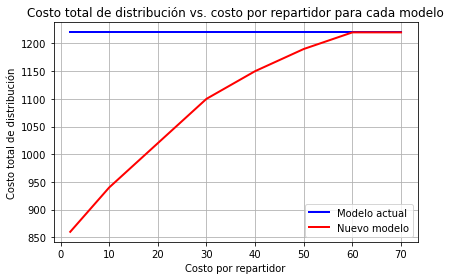
\includegraphics[width=0.6\textwidth]{costo_tot_vs_costo_rep.png}
    \caption{Costo total vs. costo por repartidor para cada modelo}
    \label{fig:mi-imagen}
\end{figure}


\begin{figure}[H] 
    \centering
    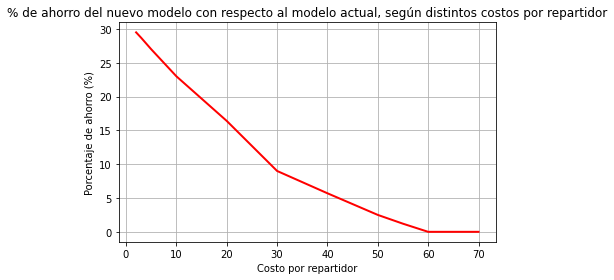
\includegraphics[width=0.8\textwidth]{porcentaje_ahorro_vs_costo_rep.png}
    \caption{Porcentaje de ahorro en costo total de distribución para el nuevo modelo en comparación con el modelo actual, según distintos costos por repartidor}
    \label{fig:mi-imagen}
\end{figure}

De estos resultados, podemos observar que si la empresa implementara el nuevo modelo y pagara 30 o menos por cada reparto realizado por repartidor, la rentabilidad de la empresa mejoraría significativamente, pues generaría un ahorro en costos de distribución mayor al 9,0\%. De hecho, si la empresa lograra conseguir repartidores que cobren 5 por viaje o menos, se reducirían los costos de entrega en un 27\% que es un ahorro muy significativo. \\
También observamos que si no se lograsen conseguir repartidores que cobren menos de 55 por viaje, entonces definitivamente no valdría la pena implementar el nuevo modelo, pues el ahorro sería prácticamente nulo. \\
Concluimos que, ante estas condiciones de este experimento, si la empresa pudiera pagar a sus repartidores una suma de 30 o menos por reparto, entonces sí le sería muy beneficiosa la aplicación del nuevo modelo. 


\subsubsection{Experimento 2: variación de densidad de clientes en la ciudad}

Todos los parámetros de este experimento se mantienen iguales que en el experimento anterior (20 clientes ubicados al azar, distancia máxima de recorrido de repartidores 5 km, un 25\% de los clientes fueron elegidos al azar para que sean quienes requieren productos refrigerados y el costo de cada tramo hecho por camión es igual a 10 veces la distancia de ese tramo), solo que ahora quedó fijo el costo por reparto de repartidor en 10 y lo que se variará será la densidad de clientes de la ciudad (número de clientes por $km^{2}$). En el caso "ciudad muy densa" se acomodarán los 20 clientes en un área de  $20/2 * 20/2$ $km^{2}$; en el caso "ciudad densa" en un área de $20 * 20$ $km^{2}$; para "ciudad moderada" un área de $20*2 * 20*2$ $km^{2}$; para "ciudad dispersa" un área de $20*4 * 20*4$ $km^{2}$; y para el caso de "ciudad muy dispersa" un área de $20*8 * 20*8$ $km^{2}$.  \\
Lo que se busca en este experimento, es ver qué tan beneficiosa sería la aplicación del nuevo modelo con respecto al modelo tradicional, en contextos de ciudades de distintas densidades de clientes por $km^{2}$. \\
\\
He aquí los resultados:

\begin{table}[H]
\centering
\resizebox{\textwidth}{!}{
\begin{tabular}{|c|c|c|c|c|}
\hline
\textbf{Densidad ciudad} & \textbf{Costo TSP} & \textbf{Costo Nuevo Modelo} & \textbf{Repartidores requeridos} & \textbf{Ahorro (\%)} \\
\hline
Muy densa & 350 & 200 & 16 & 42,9\% \\
Densa & 820 & 640 & 11 & 22,0\% \\
Moderada & 1440 & 1350 & 4 & 6,3\% \\
Dispersa & 3180 & 3010 & 3 & 5,34\% \\
Muy dispersa & 6450 & 6450 & 0 & 0\% \\
\hline
\end{tabular}
}
\caption{Comparación de costos entre metodologías para distintas densidades de clientes por $km^{2}$}
\end{table}

Como era de esperar, observamos que el uso de repartidores a pie/bicicleta resulta muy beneficioso en ciudades de alta densidad poblacional. Al ser la densidad de clientes alta, estos distan poco entre ellos. Muchas de esas distancias son menores a la distancia máxima permitida para los repartidores, por lo que muchas de las entregas podrán ser realizadas por estos, lo cual abarata muchísimo los costos de distribución de mercadería. De hecho se observa en el caso de la ciudad densa, que el 80\% de los repartos se hizo a través de repartidores. El camión debió usarse solo para llegar a 4 clientes. \\
A medida que la densidad poblacional se achica, se agrandan las distancias entre clientes y naturalmente se agrandan los costos de distribución total tanto para el modelo actual como para el nuevo modelo. Pero observando la columna "Ahorro" observamos que, a menor densidad poblacional, menos beneficio obtenemos de implementar el nuevo modelo. Esto tiene mucho sentido: a menor densidad poblacional, más grandes las distancias cliente-cliente y menos viajes factibles para hacer por repartidores, entonces es cada vez menor la diferencia que implicaría el aplicar el modelo nuevo con respecto al actual. De hecho, vemos el caso extremo en la ciudad muy dispersa, donde ningún viaje puede/conviene hacerse por repartidor, entonces el modelo nuevo no produce ninguna mejora en la rentabilidad con respecto al modelo anterior. \\
Concluimos que la aplicación del nuevo modelo puede ser útil o no, de acuerdo a la densidad de clientes que posea la ciudad. Y es especialmente útil en ciudades muy densas, donde el servicio de los repartidores será altamente utilizado. 


\subsection{Comparación metodología actual con nueva metodología} 






\end{document}